\def\theTopic{Regression Examples }
\def\dayNum{19 }

\begin{center}
{\bf {\large Regression Examples}}
\end{center}

\begin{enumerate}
\item One hundred homes\footnote{Dr. Roger
    Woodard, NCSU } were randomly \vspace{-.24in}\\ 
  \begin{minipage}{.35\linewidth} 
  sampled from a database of all
  homes in Wake County, NC.  We
  have the square footage of each home and an estimated (2008) value of
  the property.  The plot shows 98 homes with value less than \$1
  million.  \vspace*{1in}
  \end{minipage}\hfill
  \begin{minipage}{.60\linewidth}
    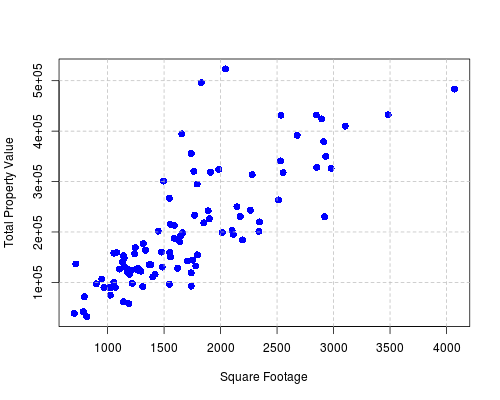
\includegraphics[width = \linewidth]{./plots/WakeCtyHomes.png}
  \end{minipage}
  \item  Describe the relationship (linear or nonlinear? positive or
    negative? strong or weak?) and give a guess at the correlation
    between area and value.
\begin{students}
 \vspace{2cm}\\
\end{students}

\begin{key}
  {\it linear, strong, positive, $r = 0.80$ }
\end{key}

  \item The equation of the least squares line is:
  $$  \widehat{value} =  -30748 + 137\times{sqft}$$
  \begin{enumerate}
  \item Compute the fitted values for homes of size 1000 and 4000 sqft.
\begin{students}
 \vspace{2cm}\\
\end{students}

\begin{key}
  {\it  for 1000: 106252  and for 4000: 517252 }
\end{key}
   \item  Mark the points on the plot and connect them to get the line
     of best fit.  \\
      Note: \verb|1.0+e05| means 1 times $10^5$, or \$100,000.  \vspace{.1in}
   \item The observed value for a 3483 sqft home is  432516.
     Compute the residual.
\begin{students}
 \vspace{2cm}\\
\end{students}

\begin{key}
  {\it  0.041}
\end{key}
   \item  Two homes in particular do not seem to fit the linear
     relationship very well.  Circle them and theorize: why might they
     have a value other than what the model predicts?  
\begin{students}
 \vspace{2cm}\\
\end{students}

\begin{key}
  {\it Size is only one variable, and it does pretty well by itself,
    but these home might have more amenities or have nicer locations
    than the others.}
\end{key}

\item Interpret the slope estimate. 
\begin{students}
 \vspace{2cm}
\end{students}

\begin{key}
  {\it Each additional square foot of house raises the estimated total
  value by \$137 }
\end{key}

\item Interpret the intercept estimate. Does its sign make sense?
\begin{students}
 \vspace{2cm}\\
\end{students}

\begin{key}
  {\it A person who has had 0 beers is estimated have BAC of -0.013
    g/dl, which does not make sense. We cannot have negative alcohol
    content in our systems. The SE of this estimate is 0.0123, so it
    is only 1 SE below zero.}
\end{key}


\end{enumerate}


\item Sixteen student volunteers\footnote{ Diez, D.M., Barr, C.D., and
    \c{C}etinkaya-Rundel, M. (2014). {\it Introductory Statistics with
    Randomization and Simulation}
     Exercise 5.28}  at \vspace{-.2in}\\ 
  \begin{minipage}{.35\linewidth}
   Ohio State University were each
  randomly assigned a number of cans of beer to drink.  Thirty minutes
  later, a police officer measured their blood alcohol 
  content (BAC) in grams of alcohol per deciliter of blood. 
  First we'll look at a plot: \vspace*{1in}

  \end{minipage}\hfill
  \begin{minipage}{.60\linewidth}
    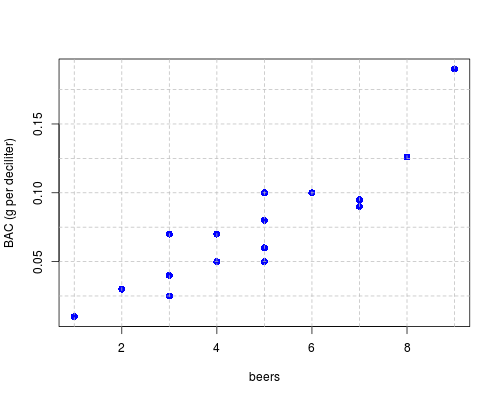
\includegraphics[width = \linewidth]{./plots/beer-BAC.png}
  \end{minipage}
\begin{enumerate}
  \item  Describe the relationship (linear or nonlinear? positive or
    negative? strong or weak?) and give a guess at the correlation
    between beers and BAC. 
\begin{students}
 \vspace{2cm}\\
\end{students}

\begin{key}
  {\it linear, strong, positive, $r = 0.90$ }
\end{key}

  \item The equation of the least squares line is:
  $$  \widehat{BAC} =  -0.013 + 0.018\times{beers}$$
  \begin{enumerate}
  \item Compute the fitted values for 2 and 9 beers.
\begin{students}
 \vspace{2cm}\\
\end{students}

\begin{key}
  {\it  for 2: 0.023  and for 9:  0.149}
\end{key}
   \item  Mark the points on the plot and connect them to get the line
     of best fit. \vspace{.2in}
   \item The observed BAC for the person who drank nine beers was 
     0.190. Compute the residual for the 9 beers person. 
\begin{students}
 \vspace{2cm}\\
\end{students}

\begin{key}
  {\it  0.041}
\end{key}
   \item  The eight beer drinker had observed BAC of 0.126. Compute
     that residual as well and explain why one residual is negative
     and the other positive.
\begin{students}
 \vspace{2cm}\\
\end{students}

\begin{key}
  {\it  -0.005. This one is negative because it's below the line. The
    9 beers person's point is above the line, so it has a positive residual.}
\end{key}

\end{enumerate}
\item Interpret the slope estimate. 
\begin{students}
 \vspace{2cm}
\end{students}

\begin{key}
  {\it Each beer a person drinks is estimated to increase BAC by 0.018 g/dl}
\end{key}

\item Interpret the intercept estimate. Does its sign make sense?
\begin{students}
 \vspace{2cm}\\
\end{students}

\begin{key}
  {\it A person who has had 0 beers is estimated have BAC of -0.013
    g/dl, which does not make sense. We cannot have negative alcohol
    content in our systems. The SE of this estimate is 0.0123, so it
    is only 1 SE below zero.}
\end{key}
\end{enumerate}\vspace*{\fill}




\end{enumerate}
 



\noindent
{\bf Assignment} \vspace{-.2in}
\begin{itemize}
\item Review for the exam
 %%  We strongly encourage you to get help in the Math Learning Center.
\end{itemize}


  %  beer <- read.csv("beers.csv")
  %  plot(BAC~beers, beer, pch = 16, col = "blue", cex = 1.3, ylab = "BAC (g per deciliter)")
  % abline(h = (1:7)*.025, lty=2, col = "grey")
  % abline(v = 1:9, lty=2, col = "grey")
  % dev.copy(png,file="plots/beer-BAC.png", height = 400, width = 500);dev.off()
  % summary(lm(BAC~beers, beer))
  
 % wakeCty <- read.csv("wakeCtyHomes.csv")
 % names(wakeCty)[c(3,8)] <- c("sqFootage","totalValue")
 % plot(totalValue ~ sqFootage, pch = 16, col = "blue", cex = 1.3, data
 %     = subset(wakeCty, totalValue < 1.0e06), xlab = "Square Footage",
 %     ylab = "Total Property Value") 
 % abline(h=(1:5)*10^5, lty=2, col = "grey")
 % abline(v=(2:8)*500, lty=2, col = "grey")
 % dev.copy(png,file="plots/WakeCtyHomes.png", height = 400, width = 500);dev.off()
 % summary(lm(totalValue ~ sqFootage, data = subset(wakeCty, totalValue
 % < 1.0e06)))
 